\documentclass{beamer}

\usepackage{parskip, setspace}
\setstretch{1.25}

\usepackage{biblatex}
\addbibresource{bib.bib}
% math formatting
\usepackage{amsmath, amsfonts, braket}
% \numberwithin{equation}{section}
% rich text
\usepackage{graphicx, caption, multimedia}
\usepackage{hyperref}
\usepackage{xcolor}
\hypersetup{
    colorlinks=true,
    linkcolor=black,  
    urlcolor=blue,
    citecolor=blue,
    pdftitle={A Survey of Computational Physics},
    pdfpagemode=FullScreen,
}

\usepackage[ruled,linesnumbered,lined,boxed,commentsnumbered]{algorithm2e}
\usepackage{animate}

\usetheme{Madrid}
\title[Computational Physics]{Computational Physics}
% \subtitle{}

\author[Chapman, Nathan]{Nathan Chapman}

\institute[CWU]
{
  Faculty of Physics\\
  Central Washington University
%   \and
%   \inst{2}%
%   Faculty of Chemistry\\
%   Very Famous University
}

\date[HPC 2024]{CS 530: High Performance Computing, Spring 2024}

\logo{
\includegraphics[height=0.5cm]{images/cwu_logo.png}}

\begin{document}

\frame{\titlepage}

\begin{frame}
    % \frametitle{<title>}

    \begin{block}{}
        \centering \Large Why do we need computers to do physics?
    \end{block}

\end{frame}

\begin{frame}
    \frametitle{An Illuminating Example - 2-Body Problem}
    \vspace{-0.75in}
    \begin{equation}
        \vec{F}_{ij} = \frac{G m_i m_j}{r_{ij}^2} \hat{r} \qquad \qquad \sum_j \vec{F}_{ij} = m_i \ddot{\vec{r}}_i
    \end{equation}

    \begin{columns}
        \column{0.5\textwidth}
        \begin{itemize}
            \item 2 masses
            \item 1 unique force
            \item 2 equations of motion in 3 dimensions
            \item 6 coupled 2nd-order ordinary differential equations
        \end{itemize}

        \column{0.5\textwidth}
        % \movie[autostart,loop,height=1.5in,width=\textwidth]{}{Orbit5.gif}
        \animategraphics[autoplay,loop,height=1.5in,width=\textwidth]{8}{orbit5/orbit5-}{0}{39}
    \end{columns}
\end{frame}

\begin{frame}
    \frametitle{An Illuminating Example - 3-Body Problem}
    \vspace{-0.75in}
    \begin{equation}
        \vec{F}_{ij} = \frac{G m_i m_j}{r_{ij}^2} \hat{r} \qquad \qquad \sum_j \vec{F}_{ij} = m_i \ddot{\vec{r}}_i 
    \end{equation}

    \begin{columns}
        \column{0.5\textwidth}
        \begin{itemize}
            \item 3 masses
            \item 3 unique forces
            \item 3 equations of motion in 3 dimensions
            \item 9 coupled 2nd-order ordinary differential equations
        \end{itemize}

        \column{0.5\textwidth}
        % \movie[autostart,loop,height=1.5in,width=\textwidth]{}{3_body.gif}
        \animategraphics[autoplay,loop,height=1.5in,width=\textwidth]{30}{3_body/3_body-}{0}{319}
    \end{columns}
\end{frame}

\begin{frame}
    \frametitle{An Illuminating Example - ``All''-Body Problem}
    \vspace{-0.75in}
    \begin{equation}
        \vec{F}_{ij} = \frac{G m_i m_j}{r_{ij}^2} \hat{r} \qquad \qquad \sum_j \vec{F}_{ij} = m_i \ddot{\vec{r}}_i 
    \end{equation}

    \begin{columns}
        \column{0.5\textwidth}
        \begin{itemize}
            \item 1.24 trillion masses
            \item $7.688\times 10^{23}$ unique forces
            \item 1.24 trillion equations of motion in 3 dimensions
            \item 3.72 trillion coupled 2nd-order ordinary differential equations
        \end{itemize}

        \column{0.5\textwidth}
        \href{https://youtu.be/JAyrpJCC_dw?si=eY7EbSKib7siokgG}{Cosmological N-Body Simulation}\cite{Heitmann_2021}
    \end{columns}
\end{frame}

\begin{frame}
    % \frametitle{<title>}

    \begin{block}{}
        \centering \Large Where do we need computers to do physics?
    \end{block}

\end{frame}

\begin{frame}
\frametitle{Problems in Computational Physics}
    \hspace{0.25in} \underline{Pillars of Physics} \hfill \underline{Computational Applications}
    \begin{itemize}
        \item <1-> Classical Mechanics \phantom{  } \rightarrowfill \phantom{  } N-Body Simulations \& Fluid Dynamics
        \item <2-> Electromagnetism \phantom{  } \rightarrowfill \phantom{  } Fringing Fields \& Antenna Radiation
        \item <3-> Thermodynamics \phantom{  } \rightarrowfill \phantom{  } Heat conduction \& Gas Diffusion
        \item <4-> Quantum Mechanics \phantom{  } \rightarrowfill \phantom{  } Electronic Structure \& Ultra-Cold Gases
        \item <5-> Relativity \phantom{  } \rightarrowfill \phantom{  } Mercury's Perihelion \& Black Hole Ray Tracing
    \end{itemize}
\end{frame}

\begin{frame}
    % \frametitle{<title>}

    \begin{block}{}
        \centering \Large Classical Mechanics
    \end{block}

\end{frame}

\begin{frame}
    \frametitle{Classical Mechanics - Mathematical Model}
    \begin{block}{Remark}
        Given the position, velocity, and forces acting on an object, its motion is completely determined.
    \end{block}
    \begin{itemize}
        \item The \emph{equation of motion}: $\sum_i \mathbf{F}_i = m \ddot{\mathbf{r}}$
        \item 2nd-order
        \item Ordinary
        \item 3 dimensions
    \end{itemize}
\end{frame}

\begin{frame}
    \frametitle{Classical Mechanics - 3-Body Equations of Motion}

    \tiny \begin{align}
        \frac{G m_2}{((x_1 - x_2)^2 + (y_1 - y_2)^2 + (z_1 - z_2)^2)^{3/2}} 
        \begin{bmatrix}
            x_2 - x_1 \\
            y_2 - y_1 \\
            z_2 - z_1
        \end{bmatrix} + 
        \frac{G m_3}{((x_1 - x_3)^2 + (y_1 - y_3)^2 + (z_1 - z_3)^2)^{3/2}} 
        \begin{bmatrix}
            x_3 - x_1 \\
            y_3 - y_1 \\
            z_3 - z_1
        \end{bmatrix} &= \begin{bmatrix}
            \ddot{x_1} \\
            \ddot{y_1} \\ 
            \ddot{z_1}
        \end{bmatrix} \\
        %
        \frac{G m_1}{((x_2 - x_1)^2 + (y_2 - y_1)^2 + (z_2 - z_1)^2)^{3/2}} 
        \begin{bmatrix}
            x_1 - x_2 \\
            y_1 - y_2 \\
            z_1 - z_2
        \end{bmatrix} + 
        \frac{G m_3}{((x_2 - x_3)^2 + (y_2 - y_3)^2 + (z_2 - z_3)^2)^{3/2}} 
        \begin{bmatrix}
            x_3 - x_2 \\
            y_3 - y_2 \\
            z_3 - z_2
        \end{bmatrix} &= \begin{bmatrix}
            \ddot{x_2} \\
            \ddot{y_2} \\ 
            \ddot{z_2}
        \end{bmatrix} \\
        %
        \frac{G m_1}{((x_3 - x_1)^2 + (y_3 - y_1)^2 + (z_3 - z_1)^2)^{3/2}} 
        \begin{bmatrix}
            x_1 - x_3 \\
            y_1 - y_3 \\
            z_1 - z_3
        \end{bmatrix} + 
        \frac{G m_2}{((x_3 - x_2)^2 + (y_3 - y_2)^2 + (z_3 - z_2)^2)^{3/2}} 
        \begin{bmatrix}
            x_2 - x_3 \\
            y_2 - y_3 \\
            z_2 - z_3
        \end{bmatrix} &= \begin{bmatrix}
            \ddot{x_3} \\
            \ddot{y_3} \\ 
            \ddot{z_3}
        \end{bmatrix}
    \end{align}

\end{frame}

\begin{frame}
    \frametitle{Classical Mechanics - Computational Model}

    \begin{columns}
        \column{0.35\textwidth}
            \begin{itemize}
                \item Finite Differences
                \item Approximates the derivative
                \item Oldest
                \item Most straightforward
            \end{itemize}
        \column{0.65\textwidth}
            \centering Central Finite Difference Coefficients
            \tiny \begin{equation}
                \begin{bmatrix}
                    1         & 1             & \ldots & 1            & 1 \\
                    -p        & -p + 1        & \ldots & p - 1        & p \\
                    (-p)^2    & (-p + 1)^2    & \ldots & (p - 1)^2    & p^2 \\
                    \vdots    & \vdots        & \vdots & \vdots       & \vdots \\
                    (-p)^{2p} & (-p + 1)^{2p} & \ldots & (p - 1)^{2p} & p^{2p} 
                \end{bmatrix}
                \begin{bmatrix}
                    a_{-p} \\
                    a_{-p + 1} \\
                    \vdots \\
                    \vdots \\
                    a_p
                \end{bmatrix} = 
                \begin{bmatrix}
                    0 \\
                    \vdots \\
                    m! \\
                    \vdots \\
                    0
                \end{bmatrix}
            \end{equation}
    \end{columns}
    \vfill
    \centering Ex. The 2-Body Problem
    \begin{equation}
        \frac{G m_1 m_2}{r_{12}^2} \hat{r}_{12} = m_1 \ddot{\mathbf{r}}_1 \implies \frac{G m_1 m_2}{r_{12, n}^2} \hat{r}_{12} = m_1 \frac{\mathbf{r}_1^{n-1} - 2 \mathbf{r}_1^n + \mathbf{r}_1^{n+1}}{h^2}
        % \frac{\partial u}{\partial t} = \frac{\partial^2 u}{\partial x^2} \implies u(x_j, t_n) = u_j^n \implies \frac{u_j^{n+1} - u_j^n}{k} = \frac{u_{j+1}^n - 2u_j^n + u_{j - 1}^n}{h^2}
    \end{equation}
\end{frame}

\begin{frame}
    \frametitle{Classical Mechanics - Computational Model}

    \begin{columns}
        \column{0.5\textwidth}
            \begin{itemize}
                \item Velocity Verlet Integration
                \item Useful for equations of motion
                \item Convserves energy
                \item The right choice for long time scales
            \end{itemize}
        \column{0.5\textwidth}
            \centering Velocity Verlet
            \begin{align*}
                n &= 0, 1, 2, 3, \ldots \\
                \mathbf{r}_1^{n + 1} &= \mathbf{r}_1^n + \dot{\mathbf{r}}_1^n \Delta t + \frac{1}{2} \ddot{\mathbf{r}} \Delta t^2 \\
                \dot{\mathbf{r}}_1^{n + 1} &= \dot{\mathbf{r}}_1^n + \frac{\ddot{\mathbf{r}}_1^n + \ddot{\mathbf{r}}_1^{n  +1}}{2}
            \end{align*}
    \end{columns}
\end{frame}

\begin{frame}
    \frametitle{Classical Mechanics - Computational Model}

    \small \begin{algorithm}[H] \DontPrintSemicolon
        \caption{N-Body Gravitational Simulation} \label{alg:nbody}
        \KwIn{Initial Positions, Initial Velocities, Masses}
        \KwOut{The trajectory of the objects}
        Discretize the equations of motion\;
        Use intial values $\mathbf{r}^0$ and $\dot{\mathbf{r}}^0$ to get $\mathbf{r}^1$ through somthing like Euler integration\;
        \While{$t^n < t^f$}{
            \For{$i \leq N$}{
                Use discretized equation of motion for object $i$ to get acceleration $\ddot{\mathbf{r}}_i^n$\;
                Use Velocity Verlet to get new velocity $\dot{\mathbf{r}}_i^{n + 1}$ and position $\mathbf{r}_i^{n + 1}$
            }
        }
    \end{algorithm}
\end{frame}

\begin{frame}
    \frametitle{Classical Mechanics - Computational Model}
    \begin{columns}
        \column{0.5\textwidth}
            \begin{itemize}
                \item Forces can be calculated in parallel
                \item N-Body simulations can benefit from CUDA implementations\cite{gpugems}
                \item ``50 times as fast as a highly tuned serial implementation (Elsen et al. 2006)''
                \item ``250 times faster than our portable C implementation''
            \end{itemize}
        \column{0.5\textwidth}
            \begin{figure}[H]
                \centering
                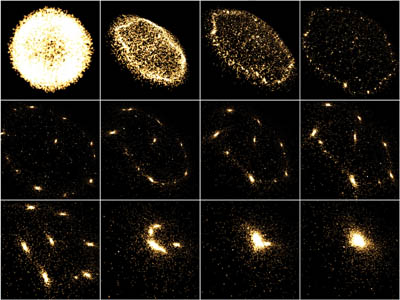
\includegraphics[width=\textwidth]{images/nbody_gpu.jpg}
                \caption*{``Frames from an Interactive 3D Rendering of a 16,384-Body System...''}
            \end{figure}
    \end{columns}
\end{frame}

\begin{frame}
    \frametitle{Classical Mechanics - Numerical Analysis}
    \begin{itemize}
        \item Discretization Error
        \item Time step $\Delta t$
        \item Verlet error $= \mathcal{O}(\Delta t^2)$ 
        \item $\Delta t \to \Delta t / 2 \implies $ error $\to$ error/4
        \item Verify results with energy conservation and energy drift
    \end{itemize}
\end{frame}

\begin{frame}
    % \frametitle{<title>}

    \begin{block}{}
        \centering \Large Electromagnetism
    \end{block}

\end{frame}

\begin{frame}
    \frametitle{Electromagnetism - Mathematical Model}
    In general, the dynamics of the electric and magnetic fields are described by Maxwell's Equations
    \begin{equation}
    \begin{aligned}
        \nabla \cdot \mathbf{E}  &= \frac{\rho}{\epsilon_0}                 & \nabla \cdot \mathbf{B}  &= 0 \\
        \nabla \times \mathbf{E} &= -\frac{\partial \mathbf{B}}{\partial t} & \nabla \times \mathbf{B} &= \mu_0 \mathbf{J} + \mu_0 \epsilon_0 \frac{\partial \mathbf{E}}{\partial t}.
    \end{aligned}
    \end{equation}
\end{frame}

\begin{frame}
    \frametitle{Electromagnetism - Mathematical Model}

    Expanded

    \footnotesize{\begin{equation}
    \begin{aligned}
        \partial_x E_x(t, \mathbf{r}) + \partial_y E_y(t, \mathbf{r}) &+ \partial_z E_z(t, \mathbf{r}) = \frac{\rho}{\epsilon_0}                 & \partial_x B_x(t, \mathbf{r}) &+ \partial_y B_y(t, \mathbf{r}) + \partial_z B_z(t, \mathbf{r})  = 0 \\
        \begin{bmatrix}
            \partial_y E_z - \partial_z E_y \\
            \partial_z E_x - \partial_x E_z \\
            \partial_x E_y - \partial_y E_x \\
        \end{bmatrix} &= -\partial_t \begin{bmatrix} B_x \\ B_y \\ B_z \end{bmatrix} & \begin{bmatrix}
            \partial_y B_z - \partial_z B_y \\
            \partial_z B_x - \partial_x B_z \\
            \partial_x B_y - \partial_y B_x \\
        \end{bmatrix} &= \mu_0 \rho \begin{bmatrix} v_x \\ v_y \\ v_z \end{bmatrix} + \mu_0 \epsilon_0 \partial_t \begin{bmatrix} E_x \\ E_y \\ E_z \end{bmatrix}
    \end{aligned}
    \end{equation}}

    \normalsize as a coupled system of eight \emph{partial} differential equations

\end{frame}

\begin{frame}
    \frametitle{Electromagnetism - Computational Model}
    \begin{columns}
        \column{0.6\textwidth}
        \begin{itemize}
            \item Finite Differences $\to$ Finite-Difference time-domain (Yee's Method)
            \item Multiple spatial dimensions $\implies$ discretized spatial mesh
            \item Also in time $\implies$ multiple runs over mesh computing gradients 
        \end{itemize}
        \column{0.4\textwidth}
        \begin{figure}[H]
            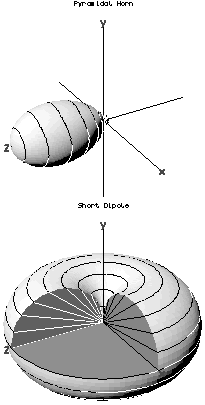
\includegraphics[height=0.7\textheight]{images/Radiation-patterns-v.png}
            \caption{Antenna radiation pattern}
        \end{figure}
    \end{columns}
\end{frame}

\begin{frame}
    \frametitle{Electromagnetism - Computational Model}

    \small \begin{algorithm}[H] \DontPrintSemicolon
        \caption{Electromagnetism Evolution}
        \KwIn{Initial State of the electromagnetic field}
        \KwOut{Final state of the electromagnetic field}
        Discretize space into mesh\;
        Discretize time into temporal chunks\;
        \For{$t_n < t_f$}{
            \ForEach{cell in mesh}{
                Calculate spatial derivatives\;
                Combine derivatives via Maxwell's Equations\;
                Get the electric and magnetic field
            }
            Calculate the time derivative of the whole mesh
        }
    \end{algorithm}

\end{frame}

\begin{frame}
    \frametitle{Electromagnetism - Numerical Analysis}

    \begin{block}{CFL Condition}
        Information in the simulation cannot travel faster than it would in reality.
    \end{block}

    \begin{itemize}
        \item Rigorously, 
        \begin{equation}
            \frac{\partial w}{\partial t} = u \frac{\partial w}{\partial x} \implies C = \frac{u \Delta t}{\Delta x} \leq C_\text{max}
        \end{equation}
        \item For explicit (time-marching) algorithms, $C_\text{max} = 1$.
        \item $C_\text{max}$ is called the \textit{Courant Number}.
        \item If the CFL condition is not met, the results are unphysical.
    \end{itemize}

\end{frame}

\begin{frame}
    % \frametitle{<title>}

    \begin{block}{}
        \centering \Large Quantum Mechanics
    \end{block}

\end{frame}

\begin{frame}
    \frametitle{Quantum Mechanics - Mathematical Model}

    The Schr{\"o}dinger equation is the quantum equation of motion
    
    \begin{equation}
        H \psi = E \psi
    \end{equation}

    and for atoms and molecules

    \small \begin{equation}
        H = -\underbrace{\sum_i \frac{\hbar}{2 m_e} \nabla_i^2}_{\text{e motion}} - \underbrace{\sum_k \frac{\hbar}{2 m_e} \nabla_k^2}_{\text{Z motion}} - \underbrace{\sum_{i,k} \frac{e^2 Z_k}{r_{ik}}}_{\text{e-Z interaction}} + \underbrace{\sum_{i < k} \frac{e^2}{r_{ik}}}_{\text{e-e interaction}} + \underbrace{\sum_{k < l} \frac{e^2 Z_k Z_l}{r_{kl}}}_{\text{Z-Z interaction}}
    \end{equation}

\end{frame}

\begin{frame}
    \frametitle{Quantum Mechanics - Computational Model}

    \begin{itemize}
        \item Molecular Mechanics $\to$ classical n-body simulation
        \item ab-initio Self-Consistent Field theory $\to$ iteratively solve the Schr{\"o}dinger equation
    \end{itemize}

\end{frame}

\begin{frame}
    % \frametitle{<title>}

    \begin{block}{}
        \centering \Large Relativity
    \end{block}

\end{frame}

\begin{frame}
    \frametitle{Relativity - Mathematical Model}

    \centering The Einstein Field Equations

    \begin{equation}
        \underbrace{G_{\mu \nu}}_\text{Curvature of Spacetime} + \underbrace{\Lambda g_{\mu \nu}}_\text{Expanding Spacetime} = \kappa \underbrace{T_{\mu \nu}}_\text{Mass and Energy}
    \end{equation}

    Actually 10 highly nonlinear, coupled partial differential equations in 4 dimensions.

\end{frame}

\begin{frame}
    \frametitle{Relativity - Computational Model}

    \begin{itemize}
        \item \href{https://youtu.be/qol-zP9W5J4?si=7ty4vfO9ceFox48e}{OpenRelativity} visualization\cite{openrelativity}
        \item The physical scenarios considered, such as binary black hole mergers\cite{blackholemerger} and ray tracing near a black hole\cite{James_2015}, yield forms of the EFEs that must be numerically solved with high-performance computing\cite{li2023solving,Andrade2021,Clough_2015}.
    \end{itemize}

\end{frame}

\begin{frame}
    \frametitle{Relativity - Results}

    \begin{figure}
        \centering
        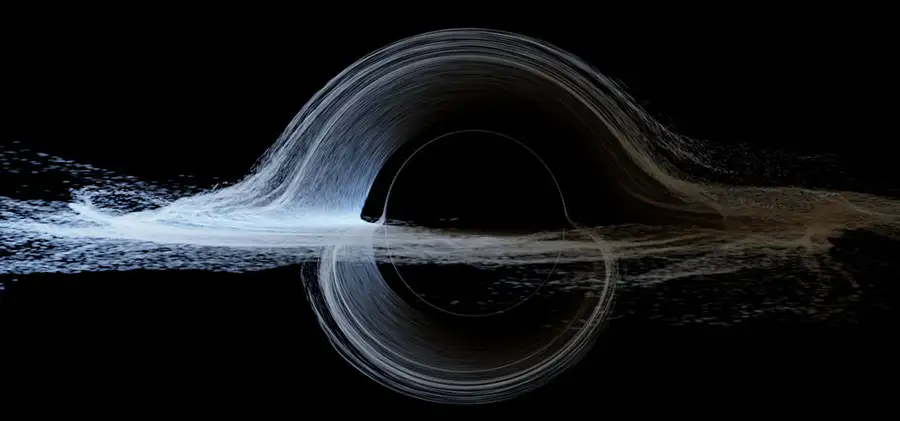
\includegraphics[width=\textwidth]{images/gargantua.png}
    \end{figure}

\end{frame}

\begin{frame}
    \frametitle{Conclusion}

    \begin{itemize}
        \item All physics can use computers
        \item Even the simplest models need computation
        \item More complex mathematical models require high-performance computing
        \item Numerical analysis is of the utmost important when developing computational models and results
    \end{itemize}

\end{frame}

% \begin{frame}
%     \frametitle{Sample frame title}
    
%     In this slide, some important text will be
%     \alert{highlighted} because it's important.
%     Please, don't abuse it.
    
%     \begin{block}{Remark}
%     Sample text
%     \end{block}
    
%     \begin{alertblock}{Important theorem}
%     Sample text in red box
%     \end{alertblock}
    
%     \begin{examples}
%     Sample text in green box. The title of the block is ``Examples".
%     \end{examples}
% \end{frame}

\nocite{*}
\begin{frame}[allowframebreaks]
\frametitle{References}
\printbibliography
\end{frame}

\end{document}